\documentclass[twocolumn]{article}
\usepackage[top=0.5in, left=0.45in, right=0.45in, bottom=0.5in]{geometry}

\usepackage{url}
% \usepackage{code}
% \usepackage{cite}
\usepackage{amsmath}
\usepackage{amssymb}
\usepackage{graphicx}
\usepackage{chessboard}

% \usepackage{chessfs}
\usepackage{adjustbox}

% Define black versions of pieces for inline use. Gross, but it works.
\newcommand{\Pawn}[1][1.3ex]{%
\adjustbox{Trim=4.3pt 2.6pt 4.3pt 0pt,width=#1,margin=0.2ex 0ex 0.2ex 0ex}{\BlackPawnOnWhite}%
}%
\newcommand{\Rook}[1][1.58ex]{%
\adjustbox{Trim=3.2pt 2.2pt 3.2pt 0pt,width=#1,raise=0ex,margin=0.1ex 0ex 0.1ex 0ex}{\BlackRookOnWhite}%
}%
\newcommand{\Knight}[1][1.85ex]{%
\adjustbox{Trim=2.3pt 2.35pt 2.5pt 0pt,width=#1,raise=-0.03ex,margin=0.14ex 0ex 0.14ex 0ex}{\BlackKnightOnWhite}%
}%
\newcommand{\Bishop}[1][1.79ex]{%
\adjustbox{Trim=2.3pt 2pt 2.3pt 0pt,width=#1,raise=-0.12ex,margin=0.1ex 0ex 0.1ex 0ex}{\BlackBishopOnWhite}%
}%
\newcommand{\Queen}[1][2.05ex]{%
\adjustbox{Trim=1.2pt 2.2pt 1.2pt 0pt,width=#1,raise=-0.08ex,margin=0.1ex 0ex 0.1ex 0ex}{\BlackQueenOnWhite}%
}%
\newcommand{\King}[1][1.95ex]{%
\adjustbox{Trim=2pt 2pt 2pt 0pt,width=#1,raise=-0.06ex,margin=0.13ex 0ex 0.13ex 0ex}{\BlackKingOnWhite}%
}%

\interfootnotelinepenalty=0

% lets me explicitly set a. or 1. etc. as enum label
\usepackage{enumitem}

\pagestyle{empty}

\usepackage{ulem}
% go back to italics for emphasis, though
\normalem

\usepackage{natbib}

\setlength{\footnotesep}{2em}

% \newcommand\comment[1]{}
\newcommand\sfrac[2]{\!{}\,^{#1}\!/{}\!_{#2}}

\begin{document} 

\title{Survival in chessland}
\author{Dr.~Tom~Murphy~VII~Ph.D.\footnote{
Copyright \copyright\ 2019 the Regents of the Wikiplia
Foundation. Appears in SIGBOVIK 2019 with the threefold
repetition of the Association for Computational Heresy; 
{\em IEEEEEE!} press, Verlag-Verlag volume no.~0x40-2A.
53 Centipawns} }

\setchessboard{showmover=false}

\newcommand\checkmate{\hspace{-.05em}\raisebox{.4ex}{\tiny\bf ++}}

\renewcommand\th{\ensuremath{{}^{\textrm{th}}}}
\newcommand\st{\ensuremath{{}^{\textrm{st}}}}
\newcommand\rd{\ensuremath{{}^{\textrm{rd}}}}
\newcommand\nd{\ensuremath{{}^{\textrm{nd}}}}
\newcommand\at{\ensuremath{\scriptstyle @}}

\date{1 April 2019}

\maketitle \thispagestyle{empty}

\begin{abstract}
CHESSMATE.
\end{abstract}

\section*{Introduction}


If you are forced to play chess to the death, you are in trouble,
because most people are not good at chess (for example, the author)
and yet want to live.\footnote{It is easy for two players to
  collaborate to produce a draw, especially by simply agreeing to a
  draw at the outset of the game (if allowed). Some tournament formats
  forbid the players from agreeing to a draw verbally before a certain
  point (e.g. 30 moves), or without the arbiter's consent, and FIDE
  rules technically do not allow a draw until both players have made a
  move (5.2.3). There are always other routes to a draw, for example
  by stalemate or repeating the same position three times.
  Collaboratively producing such situations is easy, but this strategy
  is not likely a stable equilibrium: Players can often gain a
  substantial advantage by going ``off script'' and instead trying to
  win the game. Additionally, sometimes the terms of
  chess-to-the-death do not allow the players to communicate at all
  beforehand, nor during the game. If this is the case, then it may be
  difficult to agree on the approach to drawing, let alone establish
  that this is both players' desire. Since the rules of
  chess-to-the-death can't forbid us from colluding right now as you
  read this paper, I hereby declare that the following is the correct
  approach:
\begin{enumerate}[label=\arabic*.]
  \item[1.] Nf3. This is a reasonable opening move for white (begins the R\'eti)
    which can transpose into several common systems (e.g. King's
    Indian). Since the knight can move back to g1 on the next move,
    knight moves are the fastest route to a draw by repetition. This
    has a good chance of signaling to a wise player that a draw is
    desired. The player should make this move after pondering carefully
    for some time, and then looking meaningfully into the other player's
    eyes. 
  \item[1.] \ldots Nf6. This is both a strong response for black in a real game,
    and simultaneously a signal that a draw is desired. The other
    advantage is that very weak players\cite{eloworld} may simply copy what white does.
    In doing so, they will also play this move. 
  \item[2.] Ng1?!. White moves the knight back to its starting square.
    This is a terrible move for white, but clearly signals the intention to
    draw.
  \item[2.] \ldots Ng8!. ``Fool's Draw Accepted.'' The starting position is reached
    for a second time.
  \item[3.] Nf3 Nf6. At this point the game should clearly continue repeating
    the sequence, although since we are in the start position, white has
    any number of strong opening moves available. Signaling the draw line
    and then 3. d4!? may be pyschologically devastating.
  \item[4.] Ng1 Ng8 1/2-1/2. The starting position is reached for the third
    time, which by rule\footnotemark\ is a draw.
\end{enumerate}

  Since this is one of the shortest possible routes to a draw, I
  hereby dub this line the ``Fool's Draw,'' by analogy with the Fool's
  Mate. In this line all pieces survive, which is anyway humane and
  also advantageous in the case that you are someone is simultaneously
  being one of the chesspieces to the death!

  If 1. \ldots Nc6 or another Knight's move, white can also consider
  continuing in the obvious way. However after 1. \ldots d5, black has
  refused or not noticed the draw. Fortunately, white is still in a
  good position to play the game normally (this is the main line of
  the R\'eti opening, followed by 2. c4). White can try to be more
  obvious with 2. Ng1, but if black is choosing to just play normally,
  white takes a distinct handicap by doing so.

  The biggest risk for white is that black does not play 2. \ldots Ng8
  but rather a normal move like 2. \ldots g6 (``Fool's Draw Betrayed'').
  This can happen if black is not metagaming at all (for Nf6 is a
  normal response to the normal Nf3), or if black is an exceptionally
  shrewd metagamer (tricking white into wasting two tempos with Ng1
  by pretending to be cooperating).

  Of course, this all relies on the assumption that if
  chess-to-the-death ends in a draw, the players are spared or allowed
  to repeat indefinitely. If both players are actually executed, then
  this line is truly a Fool's Draw!
}

But what if you are forced to {\it be one of the chess pieces} to the
death? That is, your little soul inhabits one of the 32 pieces or
pawns and your soul is vanquished if that piece is eliminated. Now it
doesn't matter whether you're good or bad at chess, because you don't
get to pick what happens in the game. What matters is that your piece
lives to the end of the game, when all surviving pieces are set free.
Which piece should you want to be?

In formal chess, the king can never be captured: The game ends when
the king is attacked but cannot move, and it is illegal to make a move
that leaves the king attacked. The king's death is implied, of course,
but it is seen as more poetic to end the game prior to this point.

For the sake of this question, we'll consider the the white king to
``die'' if white loses (i.e., is checkmated), and likewise for black.
Otherwise, of course, the best chances of survival would trivially be
with the two kings, since they are never formally captured. Loss
includes resignation, since most high-level games actually end once
the defeated player agrees that loss is inevitable. We can think of
this common case like king seppuku. Many games also end in time
forfeit, which is like the king's poor diet and lifestyle choices
leading to a death by natural causes.

Neither side is believed to have a decisive advantage, and many games
end in a draw, with both kings surviving. So the survival chances of a
king are likely greater than 50\%; pretty decent odds. Is it possible
that any other piece has even better chances? Let's find out---our
lives may depend on it!


\footnotetext{
  But is it?
  
  First of all, although either player is allowed to {\it claim} a
  draw after three repetitions of the same position, it is not
  automatic. However, FIDE rules do declare that the game simply ends
  in a draw upon {\it five} repetitions. Of course it is easy to
  extend the Fool's Draw to accommodate this.
  
  Second: The lichess implementation (although known to be
  buggy\cite{kingme}) does not permit a threefold repetition claim in
  this situation, which got me thinking that maybe there is some
  subtlety here. Is the starting position special somehow, not
  counting as having occurred? The relevant statute, from the FIDE
  Laws of Chess\cite{fiderules}:
  \begin{quote}
    {\bf 9.2}.\quad The game is drawn, upon a correct claim by a
    player having the move, when the same position for at least the
    third time (not necessarily by a repetition of moves):
    \begin{enumerate}[label=\alph*.]
    \item is about to appear, if he first writes his move, which
      cannot be changed, on his scoresheet and declares to the arbiter
      his intention to make this move, or
    \item has just appeared, and the player claiming the draw has the
      move.
  \end{enumerate}

  Positions are considered the same if and only if the same player has
  the move, pieces of the same kind and colour occupy the same squares
  and the possible moves of all the pieces of both players are the
  same. Thus positions are not the same if:
  \begin{enumerate}[label=\arabic*.]
  \item at the start of the sequence a pawn could have been captured
    en passant.
  \item a king or rook had castling rights, but forfeited these after
    moving. The castling rights are lost only after the king or rook
    is moved.
  \end{enumerate}
  \end{quote}
  
  So the question is, has the starting position ``appeared'' before
  white's first move? The rules are not totally clear on this point.
  Note that ``positions are considered the same'' only when the
  same player ``has the move.'' FIDE defines ``have the move'' as
  \begin{enumerate}[label=\arabic*.3.] % hack to get 1.3.
    \item A player is said to 'have the move' when his opponent's
    move has been 'made'.
  \end{enumerate}
  A strong case can therefore be made that white does not 'have the
  move' in the formal sense at the beginning of the game, since black
  has not made a move!
  
  Nonetheless, it does seem clear that white can claim a draw by
  9.2.a, by committing the move 5. Nf3 and declaring to the arbiter
  that the position is now {\it about to appear} for the third time.
  This seems unambiguously legal. }

\section{Hypotheses} \label{sec:hypotheses}

Like all good scientific research, I clearly laid out my hypothesis
and wrote down the motivation before performing the study. This helps
prevent presentation bias where the results appear more satisfactory
because they are framed as a natural conclusion from the idea that
motivated the research in the first place (when in fact, of course, if
you write the motivation after witnessing the results, backflow is
inevitable). It is also much more exciting. I literally don't know the
answer as I'm writing this, nor whether it is interesting in any way!

Here are my guesses.

\begin{itemize}
\item Black and white are probably not significantly different. That
  is, the a1 and a8 rooks probably have about the same survival
  chances (it's known that white has a slight statistical
  advantage~\cite{chesstego} but it is probably only around 1\%). So
  these guesses will be written about white's pieces.
\item The d2 and e2 pawns are very active in common openings, and
  are frequently captured as part of those openings. I think they
  are the least likely to survive overall.
\item Bishops and knights are often involved in the opening and
  midgame, and often exchanged nonchalantly. I think they all have
  relatively low survival chances.
\item Although the queen is very valuable, a queen exchange is often
  forced for games that enter the endgame.
\item Rooks tend to be late-game pieces, because they are difficult
  to get out of their corners (and at most one can be activated
  by the fastest method, castling) and are relatively valuable.
\item This leaves the non-central pawns. These are the hardest to
  predict, and they are hard to think about (at least for me) because
  when e.g. the a2 pawn recaptures the b3 pawn that it supported, I
  just think of this as the b3 pawn. Of these pawns, b2 and g2 are
  somewhat weak because they are undefended once the bishop is
  developed (cf. the famous ``poison pawn'' at b2). On the other hand,
  in the fianchetto configuration, this pawn is very strong and often
  survives the entire game without leaving the third rank. Since pawn
  chains usually progress towards the middle of the board, the a2 pawn
  is more likely to be supporting than supported. This both leaves it
  weak to capture, but prone to recapturing. Outside pawns block one's
  own rook, although for this same reason they often clear the file by
  capturing (and so survive). They are also commonly used to push into
  a well-defended king's territory (e.g. in the fianchetto); kingside
  castling is more common, so this means that the h pawns are often
  lost to this fate.
\end{itemize}

The final ranking that I committed to, from most surviving to most dead:
\pawn f, \pawn c, \pawn g, \pawn a, \pawn h, \pawn b, \rook h, \rook a,
\king, \queen, \bishop f, \knight g, \pawn e, \pawn d.

As already copped to, while the author is an aficionado and also knows
how to spell the difficult word aficionado without spell-check, he is
not good at chess. A few drinking buddies with varying chessperience
were also consulted for their wagers; these are compared to each other
and to the actual results in Section~\ref{sec:guesses}.


\section{Methodology}

To compute the chances for survival, I legally acquired 506,000,416
chess games from lichess.org. This is all of the standard variant,
rated games from Jan 2013 to November 2018, in any time format. Only
games that are completed and valid are included (about 200,000 games
did not meet this criteria). The total data size is 875 gigabytes, so
processing these took some care for efficiency and parallelism.
Fortunately, I have a computer with just an obscene number of cores
and truly excessive RAM, so you gotta use that for
something.\footnote{ To torture your own desktop computer, source code
  is available at
  \url{sourceforge.net/p/tom7misc/svn/HEAD/tree/trunk/chess/}.}

Other than that, I simply implemented the rules of chess, wrote a PGN
parser, then parsed and simulated each game. For each
of the 32 pieces in the starting position, I tracked its current
location, and whether it is alive; multiple dead pieces could
occupy the same square. At the end of the game, one of the kings is
killed if his side has lost.

For a piece, there is a single factual survival rate in these games,
given just by $\frac{\mathrm{num~survived}}{\mathrm{num~games}}$. What
we're really interested in, however, is estimating the underlying true
survival probability for each piece. In order to do this with
reasonable efficency, we divide the games into 32 separate buckets,
and count statistics separately for each. From these samples we can
then estimate variance, for example. The games are bucketized by a
deterministic hash of the White player's username. This way, if there
exist some players who are highly unusual (perhaps automated
accounts), their games are grouped together and pessimistically
represented in the variance estimate. This also helps account for
different opening preferences; the chosen opening certainly affects
the survival chances.

\begin{figure}[t]
  \begin{center}
    % To generate this pdf, I ran maketable to make
    % piece-survival.svg, then printed to PDF using Chrome, then
    % cropped it in Illustrator. Illustrator can open the SVG but
    % doesn't have the unicode chess pieces in any font I could find.
    \includegraphics[width=0.95 \linewidth]{piece-survival-export}
  \end{center}\vspace{-0.1in}
  \caption{Survival probabilities for each of the 32 pieces in standard
    chess, in 500 million games. The number is the mean survival rate
    across all samples. The vertical position of the dot is this mean
    rate, with a line drawing the span between the smallest and largest
    sample bucket (this is usually a very tiny range).
    Horizontal position is purely presentational, to avoid overlap.}
  \label{fig:piece-survival}
\end{figure}

The basic survival chances appear in Figure~\ref{fig:piece-survival}.
Indeed, many pieces are more likely to survive than the kings. Even as
black, the extremal pawns (\pawn a and \pawn h) have over a 70\%
survival rate. Across the board, the survival chances for a white
piece and its black twin are similar, usually with a small edge to
white. Notable exceptions are the \knight g (the overall most doomed
piece), and both white bishops, which die more than their
Schwarzdoppelgangers. The \pawn e is vastly more dead than \Pawn e.
Note somewhat satisfyingly that the \pawn c has the highest variance;
this was the most controversial among the drinking buddies
(Section~\ref{sec:guesses}). Note that \pawn c is the sacrificed
pawn in the popular Queen's Gambit (1. d4 d5 2. c4), where accepting
and declining the pawn are both popular and sound responses. This may
be a good example of a piece that has substantially different survival
rates in different opening preferences. Since the variance is
otherwise extremely low, I only report means for the remainder of the
paper.

Despite my impression that many games end in a draw, ties are actually
rare in the lichess database. In January 2018, only 3.8\% of games
were drawn;
% (8922275 white, 8329221 black, 682042 draw)
as a result, the survival chances for the kings are both close to
50\%. Although the database contains games in many time formats and
with all varieties of human skill (including over a thousand games by
Magnus Carlsen, the world champion and highest rated player of all
time\footnote{Although to be fair, his username ``DrDrunkenstein''
  suggests he may not play at full strength.}), blitz ($\sim\! 5$
minutes per side) and bullet ($\sim\! 1$ minute) games are
predominant. Nonetheless, the results are fairly robust across
different time formats and skill levels. In Section~\ref{sec:slices} I
show some slices of the data for comparison.


\section{Safest spaces}

The fate of each piece is to either survive or die, and it does so on
one of the 64 squares. With the same replay of the 500 million games
I also kept statistics on the fates of each piece. If being a chess
piece to the death, and possessing some influence over where your piece
moves, it may be helpful to know where to go. Even without influence,
such knowledge could help calibrate your anxiety.

% XXX using this a way to play the game

Other than the bishops---which have no legal way to reach half of the
squares---every piece ends on every square in at least a thousand
games. So we have enough samples to have reasonable confidence in our
statistics, even for the most unlikely odysseys. The least mobile
pieces are the pawns, who can technically reach any square by
promoting, but are usually confined to cones emanating from their
start squares. The overall rarest fate is for \pawn f2 to die on the
a7 square, which only happened 1,244 times (however, it survived on
this square 31,438 times). This square is actually reachable without
promoting, but it would need to capture 5 times in order to get
there, which seems quite unlikely! There may even be a hidden
achievement for reaching this square this way!
% 12 times for titled players (in new dataset too), although there are
% a few things that are even rarer, like dying on a8.
% TODO: Perhaps could find a game where this happened?!
Aside from pawns, the weirdest fate is for \knight g to die on h1,
which happened 47,307 times. Corners are of course fairly garbage for
the knight, although it is twice as likely to survive on this square.

% There may even be hidden achievements for reaching these squares!

That said, there are characteristic patterns for each of the pieces,
which make sense given their starting positions and patterns of
movement. You could probably guess the piece just by looking at one of
the heat maps below, although---spoiler alert---the piece is just
listed right there and they are in order. Two independent things are
communicated in these graphics: The chance that the piece ends the
game on some square (alive or dead), and its survival chances there.
In each map, a darker background color indicates that the piece ends
on that square more often. The shade is based on the rank (64/64 black
is most common, 63/64 black is next most common, etc.) rather than the
absolute probability, since otherwise the graphic looks boring. The
number on the square is the percentage survival of the piece when it
is last seen (either being captured or surviving to the end of the
game) on that square. The four squares with the highest survival rates
are underlined for your convenience.

\newcommand{\chessmap}[2]{\begin{center} \includegraphics[width=0.65 \linewidth]{#1} {#2} \end{center}\vspace{-0.1in}}

\chessmap{piece0}{\Rook a8}
\chessmap{piece1}{\Knight b8}
\chessmap{piece2}{\Bishop c8}
\chessmap{piece3}{\Queen d8}
\chessmap{piece4}{\King e8}
\chessmap{piece5}{\Bishop f8}
\chessmap{piece6}{\Knight g8}
\chessmap{piece7}{\Rook h8}

\chessmap{piece8}{\Pawn a7}
\chessmap{piece9}{\Pawn b7}
\chessmap{piece10}{\Pawn c7}
\chessmap{piece11}{\Pawn d7}
\chessmap{piece12}{\Pawn e7}
\chessmap{piece13}{\Pawn f7}
\chessmap{piece14}{\Pawn g7}
\chessmap{piece15}{\Pawn h7}

\chessmap{piece16}{\pawn a2}
\chessmap{piece17}{\pawn b2}
\chessmap{piece18}{\pawn c2}
\chessmap{piece19}{\pawn d2}
\chessmap{piece20}{\pawn e2}
\chessmap{piece21}{\pawn f2}
\chessmap{piece22}{\pawn g2}
\chessmap{piece23}{\pawn h2}

\chessmap{piece24}{\rook a1}
\chessmap{piece25}{\knight b1}
\chessmap{piece26}{\bishop c1}
\chessmap{piece27}{\queen d1}
\chessmap{piece28}{\king e1}
\chessmap{piece29}{\bishop f1}
\chessmap{piece30}{\knight g1}
\chessmap{piece31}{\rook h1}

\section{Guesses and slices} \label{sec:guesses}

\begin{figure}
  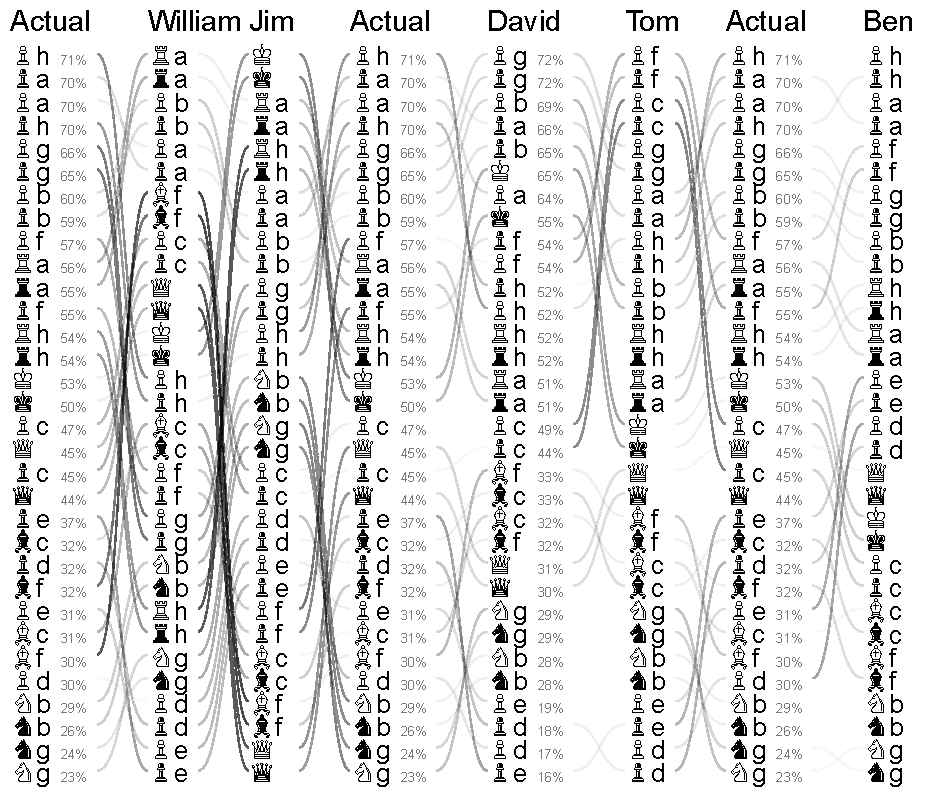
\includegraphics[width=\linewidth]{hypotheses}
  \caption{
    Piece rankings (from most surviving to most dead); either a
    human or hypothesis or the actual results across all games. 
    The {\bf actual} column appears multiple times so that each human
    gets a chance to be adjacent to it; this makes for the easiest
    visual comparison. Lines connect the same piece in adjacent columns,
    and are darker if the pairs have more different ranks.
  } \label{fig:buddies}
\end{figure}

Like all good scientific research, I explicitly compare the actual
results to the hypotheses gathered before the experiment; this is a
hygenic and humbling exercise. Figure~\ref{fig:buddies} compares the
ranking across all games (slice {\bf Actual}) to the author author
(slice {\bf Tom}) and his drinking buddies (slices {\bf Ben}, {\bf
  Jim}, {\bf David}, {\bf William}). There are a number of different
reasonable ways to measure the accuracy of this type of position; a
very simple one is the sum of the absolute differences in rank for
each piece (e.g. if in one ranking \king is \#3, and in the other \#5,
then this contributes 2 to the total error). By this metric, Ben has
the best prediction (98 error), followed by David (138) and Tom (148).
Tom and David had the most similar predictions (116) and Jim and
William the most different (312). The expected error between two
completely random permutations is about 341, so all of these guesses
are significantly better than chance. Note in the actual ranking, many
pieces have very similar survival probabilities, and many guesses are
ambivalent about groups of pieces. Weighting each rank difference
equally is therefore an oversimplification. It would have been better
to ask each participant to give probabilities, as David did; this
would give us more sensitive error metrics and more opportunities to
spend the afternoon making visualizations.

Several drinking buddies gave rationales for their hypotheses (mine
appear in Section~\ref{sec:hypotheses}).

\medskip
{\bf Ben} does not prefer to use the shift key, a typographic quirk I
replicated faithfully here even though it burns my eyes:

\begin{quote}
edge pawns almost never played til endgame let alone traded off (\pawn
h, \pawn a)

not quite sure where these should go (pb more likely to see play in
queenside minority attacks in k-side castle games?) (\pawn f, \pawn g, \pawn b)

rook play more likely to be active on q side than on k side (also the
classic Nxc7 fork in low rank play), but overall more likely to stay
tucked away compared to q (\rook h, \rook a)

i think IQP positions are more likely than not saccing e in e4 openings
but on the other hand d is often traded off in e4 openings while vice
versa is not as true (\pawn e, \pawn d)

q probably involved in many checkmates (low ranked play) or resignations
before traded off (high ranked play) (\queen)

just randomly guessing k dies in about 1/3 of games, times 1/2 for 2
sides (\king)

this pawn is a super goner (sicilian, QGA, ...) (\pawn c)

most doomed seem to be the minor pieces as i'd guess at least half of
them get traded off on c/f/3/6 or e/d/4/5 in near every game so (\bishop c, \bishop f, \knight b, \knight g)
\end{quote}

{\bf Jim} ``barely understands the rules of chess'' and ``rarely plays.'' His justifications get ``increasingly nonsensical:''

\begin{quote}
Most-to-least-survival hero tier list for chess (patch 1.0):

1.: King --- If I estimate that about 2/3rds of all regular pieces are
captured in an average game, and the probability of any non-king piece
being captured is uniform, then the king is clearly the most likely to
survive. (I'm going to break symmetry here and rank black king less
likely to survive than white king.)

2. Both Rooks --- Kept in reserve for castling purposes.

3. The A, B, G, and H pawns --- maybe people will forget to move them because they are far from the center.

4. Both Knights --- They are slippery, but they often get deep into enemy territory quickly.

5. The C,D,E,F pawns --- Moved forward to release various more important pieces $\Rightarrow$ more likely to die.

6. Both Bishops --- https://youtu.be/gDnE-5lD7w8

7. The Queen --- A high-value target, seems unlikely to survive.
\end{quote}

{\bf David} simply provided a ranking, along with survival
probabilities, in typical understated style.

\medskip
{\bf William} notes that his guesses are
``pretty much off the cuff,'' but provides some motivated reasoning:

\begin{quote}
I figure the king has got to be somewhere near the middle of the pack
since he dies in half of games featuring a winner---but with slightly
higher-than-even odds of surviving, since some games end in a draw.
I'm probably mixing up means and medians here somehow..

I'm gonna assume castling happens more often on the King's side, so
let's give Kingside Rook and F, G, and H Pawns a better shot than
their fellows on the left. But maybe it should actually be worse,
since if they die, it's because they failed to protect the king. Plus,
having heard the tip about C Pawn\footnote{I believe the ``tip'' here
  was that I described the rest of us (William was the last
  respondant) as disagreeing most on \pawn c. I think William
  misinterpreted this ``tip.''} loud and clear, I'm gonna assume that
bad boy most often becomes a new Queen, which means he gets more
survival points than the real Queen herself.

D and E Pawn are nothing but pawns, and they mostly sacrifice
themselves to the cause.

Randomizing within these constraints gives us our starting point. Then
the wildcard Bishops and Knights get randomly distributed through what
remains to come up with this final answer shown above.
\end{quote}


\subsection{Slices} \label{sec:slices}

\begin{figure}
  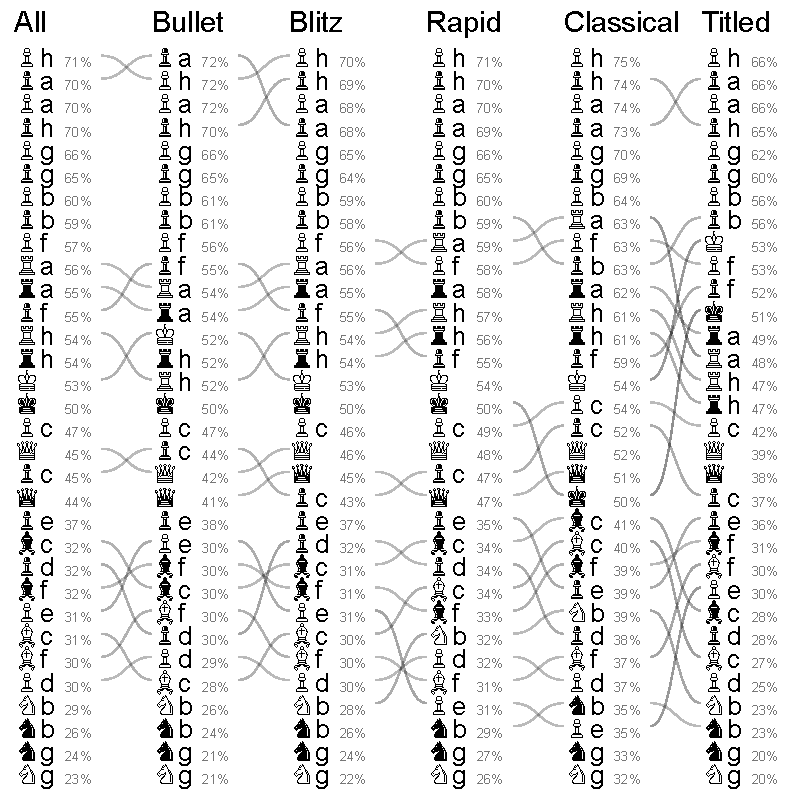
\includegraphics[width=\linewidth]{slices}
  \caption{
    Ranks and survival probabilities for different subsets of games.
    The same piece in adjacent rows is connected to highlight
    differences in the ranking, as before. The time formats all
    exhibit similar ranking with only small perturbations. Games
    including a titled player (rightmost column) are the most
    different, although we have far fewer samples in this set,
    so variance becomes significant.
  } \label{fig:slices}
\end{figure}

The survival probabilities differ depending on the conditions of the
game; Figure~\ref{fig:slices} compares some of those slices. Here the
{\bf All} slice is the same as the {\bf Actual} slice in
Figure~\ref{fig:buddies}, and consists of all acceptable games in the
database.

The {\bf titled} slice includes only games where at least one of the
players has an official title (Grandmaster, International Master, FIDE
Master, etc.\footnote{Lichess used to award the LM ``Lichess Master''
  title to notable players on the site; this title is excluded from
  the sample.}). These games have high-quality play, but far fewer
samples (``only'' 3.4 million). This set exhibits significant
variance; for example, the survival rate of \pawn c ranges from
$38$--$46\%$. This is both because of the small sample size and the
bucketization by player name; there are few enough titled players that
an individual's preference in openings and style of play moves the
values of their entire bucket. I caution against reading too much into
this column. It seems we can at least conclude that these games tend
to be much bloodier (Kings aside, survival rates are lower across the
board); top players are less likely to fall for traps early in the
game, perhaps more willing to sacrifice material, and more likely to
play into endgames where almost every piece is exchanged. If being a
chesspiece to the death, you do {\em not} want to have a Grandmaster
playing the game!

% XXX give % error % bounds?

On the other hand, the other slices all have enough samples that the
variance is minimal. These slices, {\bf bullet} (151,261,707 games),
{\bf blitz} (236,050,938 games), {\bf rapid} (98,606,558) and {\bf
  classical} (13,886,352) are different time control formats. Games on
Lichess are played with a starting clock (per side) and an increment
added to the clock after each player's move. The game is classified
according to the estimated total time: The starting time plus $40 \times$
the increment (with the idea that an average game has 40 moves per
side); this is the same formula that Lichess uses. A bullet game is
when the total time per side is between 30~seconds and 3~minutes;
blitz is between 3 and 8~minutes; rapid is between 8 and 25~minutes;
classical is any more than this (including untimed games). Each of
these slices has enough samples that the variance is very low.
Here we see that the ranking is rather stable across the range of
time formats, which was not what I expected. This should increase
our confidence that the results are really inherent to chess, not
just the particulars of this data set.


% Battle chess
% Feminist game 

\bibliography{chess}{}
\bibliographystyle{plain}

\end{document}
